\section{Swizzles}\label{sec:swizzle}

Shared-memory layouts in CUTLASS kernels are \emph{swizzled}: offsets are permuted by an XOR
pattern so that the accesses of a warp fall into distinct memory banks. C++ CuTe models this by a
function object \code{Swizzle<B,M,S>} and by \code{ComposedLayout}, a triple (swizzle, offset,
layout) that stands for the function $c\mapsto\sigma(o+f(c))$~\cite{cutedocs}; PyCuTe instead
gives layouts strides in $\F_2$~\cite{cecka2026,pycute}. Apart from the identity, a swizzle is not
additive for integer addition, so a swizzled layout is in general not a layout in the sense of
\cref{sec:background}. This section shows
that swizzles nevertheless belong to the carry calculus. Offsets carry two group laws, integer
addition and bitwise XOR; a swizzle is a layout for the second; and the two laws differ exactly
by the carries of the binary radix, which \cref{thm:carry} keeps account of.

\subsection{A swizzle is a layout for XOR}

For $x\in\N$ let $\bit_b(x)\in\{0,1\}$ be its $b$-th binary digit and
$\operatorname{supp}(x)=\{b:\bit_b(x)=1\}$; $\oplus$ is bitwise XOR. Let
$\beta\colon\N\to\F_2^{(\N)}=\bigoplus_b\F_2e_b$, $\beta(x)=\sum_b\bit_b(x)\,e_b$, be the binary
expansion; it is a bijection that turns $\oplus$ into addition. By \cref{def:layout}, $\beta$ is
the function of the layout $\lay{(2,2,\dots)}{(e_0,e_1,\dots)}$ with values in $\F_2^{(\N)}$
(with $k$ modes for offsets below $2^k$). Its jumps are $e_b-2e_{b-1}=e_b$ at the scales $2^b$,
$b\ge1$, and \cref{thm:carry} for this layout is the equation of the binary adder,
\begin{equation}\label{eq:adder}
 \beta(x+y)=\beta(x)+\beta(y)+\sum_{b\ge1}c_b(x,y)\,e_b,
 \qquad\text{i.e.}\qquad x+y=x\oplus y\oplus(\text{carry word}).
\end{equation}

\begin{definition}[swizzle]\label{def:swizzle}
A \emph{pairing} $\pi$ is a finite set of pairs $(y\to z)$ of bit positions in which no position
occurs twice. Its \emph{swizzle} $\sigma_\pi\colon\N\to\N$ replaces, for every pair, bit $z$ by
$\bit_z\oplus\bit_y$:
\[ \sigma_\pi(x)=x\oplus\bigoplus_{(y\to z)\in\pi}\bit_y(x)\,2^z . \]
CuTe's \code{Swizzle<B,M,S>}, with $B,M\ge0$ and $|S|\ge B$, is the pairing
$\{(M+S+i\to M+i):i<B\}$ if $S>0$ and $\{(M+i\to M+|S|+i):i<B\}$ if $S<0$: a field $Y$ of $B$
consecutive bits is XOR-ed into a field $Z$ at distance $|S|$ (``\code{ZZZ \^{}= YYY}''); for $B=0$
the pairing is empty and the swizzle is the identity. We put $T=M+B+|S|$, the first bit position
above both fields.
\end{definition}

\noindent The C++ functor keeps its two masks as $32$-bit signed integers. It computes $\sigma_\pi$
as long as both fields lie within bits $0$--$30$, which we assume when we speak of CuTe's swizzles;
a field that reaches bit $31$ is sign-extended against a $64$-bit offset, and then, for instance,
\code{Swizzle<1,30,1>} is no longer an involution.

\begin{example}[the 128-byte swizzle]\label{ex:sw128}
\code{Swizzle<3,4,3>} acts on byte addresses. A block of $1024$ bytes is seen as $8$ rows of
$128$ bytes, each row as $8$ chunks of $16$ bytes; the chunk index $z$ (bits $4$--$6$) is replaced
by $z\oplus y$, where $y$ (bits $7$--$9$) is the row index. For fixed $y$ the map $z\mapsto z\oplus y$
permutes the chunks of a row, so each row still occupies its own $128$ bytes; for fixed $z$ the map
$y\mapsto z\oplus y$ is a bijection as well. In other words $(y,z)\mapsto z\oplus y$ is a Latin
square: a column of the tile, which without the swizzle sits at the same chunk position in every
row (and so, when the row length is a multiple of the bank period, in the same banks), is spread
over all $8$ chunk positions (\cref{fig:swizzle}).
\end{example}

\begin{figure}[t]\centering
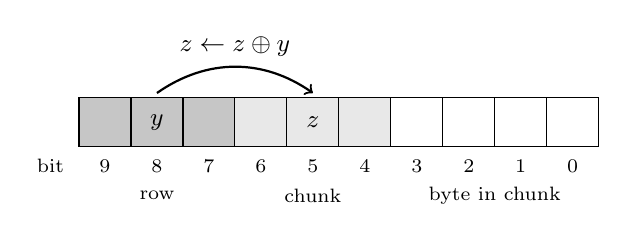
\begin{tikzpicture}[x=0.66cm,y=0.62cm,font=\small,baseline=(current bounding box.center)]
  \fill[gray!45] (0,0) rectangle (3,1);
  \fill[gray!18] (3,0) rectangle (6,1);
  \foreach \b in {0,...,9} {
    \draw (9-\b,0) rectangle ++(1,1);
    \node[font=\scriptsize] at (9.5-\b,-0.4) {\b};
  }
  \node at (1.5,0.5) {$y$};
  \node at (4.5,0.5) {$z$};
  \node[font=\scriptsize] at (1.5,-1.0) {row};
  \node[font=\scriptsize] at (4.5,-1.0) {chunk};
  \node[font=\scriptsize] at (8,-1.0) {byte in chunk};
  \node[anchor=east,font=\scriptsize] at (-0.1,-0.4) {bit};
  \draw[->,thick] (1.5,1.1) to[bend left=35] node[above,midway] {$z\leftarrow z\oplus y$} (4.5,1.1);
\end{tikzpicture}
\qquad\qquad
$\begin{array}{c|cccc}
 y\backslash z&0&1&2&3\\\hline
 0&0&1&2&3\\ 1&1&0&3&2\\ 2&2&3&0&1\\ 3&3&2&1&0
\end{array}$
\caption{Left: the bit fields of a byte address under \code{Swizzle<3,4,3>} (\cref{ex:sw128}); the
field $Y$ (dark) is XOR-ed into the field $Z$ (light). Right: the chunk position $z\oplus y$ of
logical chunk $z$ in row $y$ for two-bit fields; every row and every column is a permutation.}
\label{fig:swizzle}
\end{figure}

\begin{lemma}[structure of a swizzle]\label{lem:swizzle}
Let $\sigma=\sigma_\pi$.
\begin{enumerate}[label=(\alph*),itemsep=1pt]
\item $\sigma$ is an involution of $\N$, and
 $\sigma(x)=x+\sum_{(y\to z)\in\pi}2^z\,\bit_y(x)\bigl(1-2\,\bit_z(x)\bigr)$.
\item $\sigma(x\oplus x')=\sigma(x)\oplus\sigma(x')$. Equivalently $\beta\circ\sigma=\Lambda\circ\beta$
 for the linear map $\Lambda=1+N$ with $Ne_y=e_z$ for $(y\to z)\in\pi$ and $Ne_b=0$ otherwise.
 Hence $\beta\circ\sigma$ is the function of the layout
 $\lay{(2,2,\dots)}{(\Lambda e_0,\Lambda e_1,\dots)}$ with values in $\F_2^{(\N)}$.
\item If all positions of $\pi$ are below $T$, then $\sigma(x+2^Tq)=\sigma(x)+2^Tq$ for $x<2^T$.
 If all are at least $M$, then $\sigma(x)\equiv x\pmod{2^M}$.
\item If $z<y$ for every pair (as for $S>0$), then $\sigma$ permutes $\rng{2^t}$ for every $t\ge0$.
\end{enumerate}
\end{lemma}
\begin{proof}
Only the bits $z$ change, and the bits $y$ do not; so applying $\sigma$ twice restores every bit.
For two bits, $(b\oplus a)-b=a(1-2b)$, which gives the formula. (b) holds because every bit of
$\sigma(x)$ is an $\F_2$-linear function of the bits of $x$. (c) and (d) are read off the
definition; for (d), if $x<2^t$ then the pairs with $y\ge t$ are inactive and those with $y<t$
change a bit below $t$.
\end{proof}

\noindent So a swizzle \emph{is} a layout, as soon as offsets are added by XOR. What makes
swizzled layouts delicate is that the layout underneath adds its contributions as integers.

\subsection{Swizzled layouts}

A \emph{swizzled layout} is a triple $(\sigma,o,f)$ of a swizzle, an offset $o\in\N$ and an
$\N$-valued layout $f=\lay TR$ with $T=(t_0,\dots,t_{n-1})$, $R=(r_0,\dots,r_{n-1})$; its function
is $h(c)=\sigma(o+f(c))$. It is the composite of the $\F_2$-valued layout of
\cref{lem:swizzle}(b) with an integer layout, so \cref{thm:defect} applies to it.

\begin{theorem}[composition formula for swizzled layouts]\label{thm:swzcomp}
For every $c\in\rng{t_0}\times\dots\times\rng{t_{n-1}}$,
\begin{align*}
 \sigma\Bigl(o+\sum_jc_jr_j\Bigr)&=\sigma(o)\;\oplus\bigoplus_{j\,:\,c_j\text{ odd}}\sigma(r_j)
 \;\oplus\bigoplus_{b\ge1\,:\,\Cdef_b(c)\text{ odd}}\sigma(2^b),\\
 \Cdef_b(c)&=\floor{\frac{(o\bmod2^b)+\sum_jc_j\,(r_j\bmod2^b)}{2^b}} .
\end{align*}
\end{theorem}
\begin{proof}
Let $A$ be the layout of \cref{lem:swizzle}(b), and let $B'$ be the inner layout with shape
$(2,t_0,\dots,t_{n-1})$ and strides $(o,r_0,\dots,r_{n-1})$. Apply \cref{thm:defect} to $A$ and
$B'$ at the coordinate $(1,c)$. The jump of $A$ at scale $2^b$ is
$\Lambda e_b=\beta(\sigma(2^b))$, and in $\F_2^{(\N)}$ a multiple $m\cdot v$ is $v$ or $0$
according to the parity of $m$.
\end{proof}

A swizzled layout is thus XOR-linear in the coordinates \emph{up to the parity of the binary
carries} that the inner layout produces. Two cases in which it reduces to a layout over a single
group can be described exactly.

\begin{definition}\label{def:bitdisjoint}
A layout $\lay TR$ with values in $\N$ is \emph{bit-disjoint} if every mode with non-zero stride
has a size that is a power of two, and the numbers $2^b\,r_j$ ($0\le b<\log_2t_j$, $r_j\ne0$)
have pairwise disjoint supports. Its \emph{binary refinement} replaces every mode of size
$t_j\ge2$ with $r_j\neq0$ by $\log_2t_j$ binary modes with these numbers as strides, and keeps the
unit modes and the modes with stride $0$ (giving them the stride $0$); if
$\rho_1,\dots,\rho_p$ are the strides of its binary modes and $c_1,\dots,c_p\in\{0,1\}$ their
coordinates, then $f(c)=\bigoplus_lc_l\rho_l$.
\end{definition}
\noindent Compact layouts with power-of-two mode sizes are bit-disjoint: they permute the binary
digits. So is every layout obtained from one by dropping modes, e.g.\ the tiles of a power-of-two
array.

\begin{corollary}[XOR-linear swizzled layouts]\label{cor:xorlinear}
For a swizzle $\sigma$, the map $c\mapsto\sigma(f(c))$ is the function of an $\F_2$-valued
layout over a by-mode refinement of $T$ if and only if $f$ is bit-disjoint. In that case it is the
layout over the binary refinement with the strides $\beta\sigma(\rho_1),\dots,\beta\sigma(\rho_p)$
on the binary modes and $0$ on the others.
\end{corollary}
\begin{proof}
If $f$ is bit-disjoint, no carries occur on the binary refinement and \cref{thm:swzcomp} gives
the claim. Conversely, in an $\F_2$-valued layout a mode of size at least $3$ with stride $v$
takes the value $2v=0$ at its coordinate $2$; as $\sigma$ is injective and $\sigma(0)=0$, such a
mode of the refinement has integer stride $0$. Hence every mode of $f$ with $r_j\neq0$ is refined
into binary modes, so $t_j$ is a power of two; and for two binary modes with strides
$\rho,\rho'$, additivity gives $\sigma(\rho+\rho')=\sigma(\rho)\oplus\sigma(\rho')=\sigma(\rho\oplus\rho')$,
so $\rho+\rho'=\rho\oplus\rho'$, i.e.\ the supports are disjoint.
\end{proof}

\noindent When all mode sizes of $f$ are powers of two, the layouts of \cref{cor:xorlinear} are
linear layouts in the sense of Triton and $\F_2$-stride layouts in the sense of PyCuTe, where a
mode of size $2^p$ with $\F_2$-stride $d$ is read as $p$ binary modes with strides
$d,2d,\dots,2^{p-1}d$. For instance, in PyCuTe's notation,
\[ \text{\code{Swizzle<3,0,3>}}\circ(8,8):(1,8)\;=\;(8,8):(\mathrm F_2(1),\mathrm F_2(9)). \]
Not every layout of that kind arises in this way: in $(2,2):(\mathrm F_2(1),\mathrm F_2(1))$ two
modes have the same non-zero stride, whereas the strides $\beta\sigma(\rho_l)$ of the corollary
are pairwise distinct, $\sigma$ being injective and the $\rho_l$ having disjoint supports. The
corollary says exactly when a swizzled layout with offset $0$ is one of them.

The second case is the one CuTe needs when a swizzled tensor is sliced: with some coordinates
fixed, the rest may be an ordinary layout again, possibly with negative strides.

\begin{theorem}[decay to an ordinary layout]\label{thm:decay}
Let $f$ be bit-disjoint with binary refinement strides $\rho_1,\dots,\rho_p$, and let
$\operatorname{supp}(o)$ be disjoint from every $\operatorname{supp}(\rho_l)$. The following are
equivalent.
\begin{enumerate}[label=(\roman*),itemsep=1pt]
\item $c\mapsto\sigma(o+f(c))-\sigma(o)$ is the function of a $\Z$-valued layout over the binary
 refinement of $T$.
\item No pair of $\pi$ is split between two modes: there are no $(y\to z)\in\pi$ and $l\neq m$
 with $y\in\operatorname{supp}(\rho_l)$ and $z\in\operatorname{supp}(\rho_m)$.
\end{enumerate}
In that case the strides are $\delta_l=\sigma(o+\rho_l)-\sigma(o)$. In particular a mode that
moves only the bit $z$ of a pair has stride $+2^z$ or $-2^z$ according as $\bit_y(o)$ is $0$ or
$1$, and a mode that moves only the bit $y$ has stride $2^y+2^z$ or $2^y-2^z$ according as
$\bit_z(o)$ is $0$ or $1$.
\end{theorem}
\begin{proof}
For $c\in\{0,1\}^p$ we have $o+f(c)=o\oplus\bigoplus_lc_l\rho_l$, hence
$\sigma(o+f(c))=u\oplus\bigoplus_lc_lv_l$ with $u=\sigma(o)$ and $v_l=\sigma(\rho_l)$. Let
$V_l=\operatorname{supp}(v_l)$; a position $z$ of a pair $(y\to z)$ lies in $V_l$ iff exactly
one of $y,z$ lies in $\operatorname{supp}(\rho_l)$, and all other positions of $V_l$ are those of
$\operatorname{supp}(\rho_l)$. As the supports of the $\rho_l$ are disjoint, (ii) says that the
sets $V_l$ are pairwise disjoint. XOR-ing $v_l$ into a word $w$ flips its bits in $V_l$ and
changes its value by $\Delta_l(w)=\sum_{b\in V_l}(1-2\,\bit_b(w))\,2^b$. If the $V_l$ are pairwise
disjoint, the flips for the other modes do not touch $V_l$, so $\Delta_l(w)=\Delta_l(u)=\delta_l$
throughout and $\sigma(o+f(c))=u+\sum_lc_l\delta_l$. If $V_l\cap V_m\neq\emptyset$, the value at
$c=e_l+e_m$ differs from $u+\delta_l+\delta_m$ by
$-2\sum_{b\in V_l\cap V_m}(1-2\,\bit_b(u))\,2^b$, a signed sum of distinct powers of two, which is
not zero. The two special cases follow from \cref{lem:swizzle}(a).
\end{proof}

\noindent To apply the theorem, write each remaining mode as binary modes, mark the bits that
each of them moves, and look for a pair $(y\to z)$ whose two bits are moved by different binary
modes. Under the hypotheses of the theorem the strides $\delta_l$ are the ones the CuTe source
uses when it replaces a slice by an ordinary layout; the source assumes, as we do, that the bits
moved by the remaining layout are not set in the offset. Without the two disjointness hypotheses
the question is still decidable. By \cref{prop:additive} and \cref{lem:forced}, $h-h(0)$ is a
layout over a by-mode refinement $T'$ of $T$ if and only if it is $T'$-additive, and its strides
are then its values at the units; such a $T'$ exists if and only if
$\spec(h-h(0))\cup\Sc(T)\cup\{|T|\}$ is a chain under divisibility (\cref{thm:exact}(iv)).

\begin{example}\label{ex:decay}
Let $f=(4,2):(1,4)$ and $\sigma$ be \code{Swizzle<1,1,1>}, the pairing $\{2\to1\}$. The function
of $(\sigma,0,f)$ is $(0,1,2,3,6,7,4,5)$; the pair is split between the two modes, and this is
not a layout. Fix the second coordinate to $1$: then $o=4$, the remaining mode $4:1$ has the
binary refinement $(2,2):(1,2)$, the pair is no longer split, and
$\delta=(\sigma(5)-\sigma(4),\,\sigma(6)-\sigma(4))=(1,-2)$. The slice is the layout
$(2,2):(1,-2)$ shifted by $\sigma(4)=6$, with values $6,7,4,5$---which is what C++ CuTe returns for
this slice.
\end{example}

\subsection{Operations on swizzled layouts}\label{sec:swzops}

CuTe extends its operations to swizzled layouts by acting on the inner layout. We state when each
rule is valid; \cref{sec:testing} reports what the implementations do outside these conditions.

\paragraph{Composition on the right, division, products.}
$\sigma\circ(o+f)\circ B=\sigma\circ(o+f\circ B)$ holds whenever $f\circ B$ exists, so
\code{composition}, \code{logical\_divide} and their relatives reduce to the inner layout and to
\cref{sec:composition,sec:complement}. For products one needs in addition that copies of a tile
are translates of each other: by \cref{lem:swizzle}(c),
$\sigma(o+f(c)+q)=\sigma(o+f(c))+q$ if $o+f(c)<2^T$ and $2^T\mid q$; the atom of
\cref{ex:sw128}, for instance, covers exactly one period $2^T=1024$ of its swizzle.

\paragraph{Slicing.}
Let $P(x)=\sum_b\bit_b(x)\,2^b$, the sum over the positions of $\pi$, and $P^\perp(x)=x-P(x)$; then
$\sigma=\sigma\circ P+P^\perp$. For \code{Swizzle<B,M,S>} both $P$ and $P^\perp$ are layout
functions over the shape $(2^M,2^B,2^{|S|-B},2^B,\infty)$, the last mode being unbounded; their
strides are $(0,2^M,0,2^{M+|S|},0)$ and $(1,0,2^{M+B},0,2^T)$. The CuTe source builds these two
layouts under the names \code{swizzle\_only\_zy} and \code{swizzle\_anti\_zy}. Their jumps can
only sit at the field boundaries $2^M$, $2^{M+B}$, $2^{M+|S|}$ and $2^T$ (some of which may
coincide).

\begin{proposition}[offset bookkeeping]\label{prop:fields}
Let $a,s\in\N$ and let $o=P(o)$ with $\operatorname{supp}(o)\cap\operatorname{supp}(P(a))=\emptyset$.
If the addition $o+a+s$ produces no carry across a field boundary, then
\[ \sigma(o+a+s)=\sigma\bigl((o\oplus P(a))+s\bigr)+P^\perp(a). \]
\end{proposition}
\begin{proof}
By \cref{thm:carry} applied to $P$ and $P^\perp$, both are additive on $o+a+s$ and on
$(o\oplus P(a))+s$ (the residues of $o\oplus P(a)=o+P(a)$ at a boundary are at most those of
$o+a$). Hence
$\sigma(o+a+s)=\sigma(o+P(a)+P(s))+P^\perp(a)+P^\perp(s)=\sigma((o\oplus P(a))+s)+P^\perp(a)$.
\end{proof}

\noindent This is the rule of \code{slice\_and\_offset}, with $a$ the contribution of the fixed
coordinates and $s=f_s(c)$ that of the remaining ones: the field bits of $a$ are XOR-ed into the
offset kept inside the swizzle, the other bits are moved to the pointer, and the remaining
layout is replaced by an ordinary one when no pair has both of its bits active---a sufficient
condition for \cref{thm:decay}(ii). The hypotheses hold when the swizzled layout starts from the
offset $0$ and its inner layout is bit-disjoint: the offset is then a sum of contributions of
modes that have been sliced away and shares no bit with the remaining ones. They can fail
otherwise---for an inner layout that is not bit-disjoint, and also for a swizzled layout that is
constructed with an offset overlapping the bits of its layout (\cref{tab:swzex})---and the
source, which checks the divisibility conditions of the two projections, does not test them.

\paragraph{Pushing a swizzle through a layout.}
\code{composition(a, Swizzle)} must rewrite $a\circ\sigma$, a swizzle of the \emph{indices} of
$a$, as $\sigma'\circ a$, a swizzle of its offsets.

\begin{proposition}[transport]\label{prop:transport}
Let $N=2^n$, let $a\colon\rng N\to\N$, and let $\pi$ be a pairing with all positions below $n$.
Let $\pi'$ be a pairing and $(y\to z)\mapsto(y'\to z')$ a bijection $\pi\to\pi'$ such that for all
$x\in\rng N$: {\rm(i)} $\bit_{y'}(a(x))=\bit_y(x)$ and $\bit_{z'}(a(x))=\bit_z(x)$; {\rm(ii)}
$a(x+2^z)=a(x)+2^{z'}$ whenever $\bit_z(x)=0$. Then $a\circ\sigma_\pi=\sigma_{\pi'}\circ a$ on
$\rng N$.
\end{proposition}
\begin{proof}
$\sigma_\pi(x)$ arises from $x$ by flipping the bits $z$ with $\bit_y(x)=1$. By (ii) each flip
changes the value of $a$ by $(1-2\,\bit_z(x))\,2^{z'}$, so by (i)
$a(\sigma_\pi(x))=a(x)+\sum_{(y'\to z')}2^{z'}\,\bit_{y'}(a(x))\,(1-2\,\bit_{z'}(a(x)))=\sigma_{\pi'}(a(x))$
by \cref{lem:swizzle}(a).
\end{proof}

\noindent The hypotheses hold when $a$ is bit-disjoint and sends the index bits $y,z$ to the
offset bits $y',z'$. CuTe takes for $\sigma'$ the swizzle whose two masks are the images $a(Y)$
and $a(Z)$ of the masks of $\sigma$. That determines the two fields but not the bijection between
the pairs, nor does it test (i) and (ii): if $a$ reverses the bits of one field only, or lets
other modes touch the fields, the result is wrong (\cref{tab:swzex}). The same rule is used by
\code{right\_inverse} of a swizzled layout.

\paragraph{Merging, casting, cosize.}
If $\pi\triangle\pi'$ is again a pairing, then
$\sigma_\pi\circ\sigma_{\pi'}=\sigma_{\pi\triangle\pi'}$: indeed
$\Lambda_\pi\Lambda_{\pi'}=1+N_\pi+N_{\pi'}+N_\pi N_{\pi'}$, common pairs cancel in
$N_\pi+N_{\pi'}$, and $N_\pi N_{\pi'}\neq0$ would require a position that is a $z$ of $\pi'$ and a
$y$ of $\pi$, which would occur twice in $\pi\triangle\pi'$. (Without the hypothesis the composite
need not be a swizzle: for $\pi=\{2\to1\}$ and $\pi'=\{1\to0\}$ it is not an involution.) CuTe
merges two swizzles of equal shift $S$ by XOR-ing their masks, and accepts the result if the two
new masks are the fields of a \code{Swizzle}. This is sound. Suppose a position $b$ were a $z$
of $\pi'$ and a $y$ of $\pi$. A field has at most $|S|$ consecutive bits and so cannot contain two
positions at distance $|S|$; hence $b$ lies in neither $Y'$ nor $Z$, and therefore in both new
masks $Y\triangle Y'$ and $Z\triangle Z'$. Their union then has fewer bits than the two disjoint
fields of a swizzle, and the merge is rejected.

For casting, let $\sigma^{(n)}$ be the swizzle with the pairs $(y-n\to z-n)$ for the pairs
$(y\to z)$ of $\sigma$ with $y,z\ge n$; this is CuTe's \code{upcast} by $2^n$. Then
$\floor{\sigma(x)/2^n}=\sigma^{(n)}(\floor{x/2^n})$ holds whenever $2^n\mid x$, and it holds for
all $x$ if and only if no pair has $y<n\le z$ (in particular if $z<y$ for every pair).

Finally CuTe defines the \code{cosize} of a swizzled layout as that of its inner layout. By
\cref{lem:swizzle}(d) this is correct when $S>0$ and the image of $o+f$ is an interval
$\rng{2^t}$; in general the largest offset of a swizzled layout can be larger or smaller:
\code{Swizzle<1,0,1>} applied to $2:2$ takes the values $0,3$, and applied to the compact layout
$3:1$ the values $0,1,3$.

\paragraph{$\F_2$ strides.}
In PyCuTe a swizzled layout is an $\F_2$-stride layout $A$. If the mode sizes of $A$ are powers
of two, $A$ is an $\F_2$-linear function of the binary digits of its index, as in
\cref{lem:swizzle}(b)---on its domain, and beyond it in PyCuTe's carry-less continuation of the
last mode---and \cref{thm:swzcomp} applies: the composite with an integer layout $B$
is XOR-linear over the binary refinement of $B$ when the binary carries produced by $B$ cancel in
parity, in particular whenever $B$ is bit-disjoint. \code{composition(A, B)} applies the per-mode
rule of \cref{sec:cute-rule} with carry-less arithmetic and does not test this, so that modes
interfere as in \cref{sec:deviations}. For example
$(8,8):(\mathrm{F}_2(1),\mathrm{F}_2(11))\circ(2,2):(2,2)$ is returned as
$(2,2):(\mathrm{F}_2(2),\mathrm{F}_2(2))$, with value $0$ instead of $4$ at the coordinate
$(1,1)$: $2+2$ carries, $2\oplus2$ does not. If $A$ has a mode whose size is not a power of two,
the carries of that radix matter as well:
$(3,2):(\mathrm{F}_2(1),\mathrm{F}_2(4))\circ(2,2):(1,2)$ is returned as
$(2,2):(\mathrm{F}_2(1),\mathrm{F}_2(2))$, with value $3$ instead of $4$ at $(1,1)$, although
$1+2$ produces no binary carry.
